\section{任务级功能需求模型与职业重新定义}
\label{sec:task_level_model}

\subsection{任务级功能需求模型（替代职业级岗位需求）}
\subsubsection{建模目标与符号}
\label{sec:notation}
我们不预测职业级岗位数量，而是预测在GenAI采纳下职业的\emph{任务组成}如何演化，以及与每个任务相关的\emph{人力劳动需求}如何随时间变化。核心主张是，当一个职业的基线任务束中足够大的部分变得可忽略不计时，该职业的性质已经改变，应被重新定义（确切的新职位名称不是模型的核心）。

考虑一个职业 $i$ 分解为任务 $j=1,\dots,J_i$。对于每个任务，我们假设以下输入已经通过任务DNA和权威重标记流程构建完成：
\begin{itemize}
  \item 基线任务权重 $w_{ij}(0)$，满足 $\sum_{j} w_{ij}(0)=1$。
  \item 替代分数 $s_{ij}\in[0,1]$：GenAI能够在多大程度上减少任务 $j$ 的人力努力。
  \item 增强分数 $c_{ij}\in[0,1]$：GenAI能够在多大程度上扩展与任务 $j$ 相关的\emph{功能}范围/需求。
  \item 采纳曲线 $A(t)\in[0,1]$：时刻 $t$ 的GenAI采纳比例/强度（情景驱动）。
\end{itemize}

我们引入四个状态变量：
\begin{align*}
Q_i(t) &:\ \text{职业 } i \text{ 的整体功能输出需求指数},\\
\ell_{ij}(t) &:\ \text{任务 } j \text{ 的劳动强度（单位输出的人力努力）},\\
w_{ij}(t) &:\ \text{时变任务劳动份额（任务结构）},\\
D_{ij}(t) &:\ \text{任务 } j \text{ 的人力劳动需求指数}
\end{align*}
直观上，$s_{ij}$ 控制人力努力对任务变得不必要的速度（自动化渠道），而 $c_{ij}$ 控制整体功能需求可以扩张的程度（规模化渠道）。这些是不同的机制，不会强制抵消。

\subsubsection{双渠道动力学：自动化与规模化}
\label{sec:two_channel}

\paragraph{(a) 自动化渠道：替代降低劳动强度。}
我们假设随着GenAI采纳增加，替代分数更高的任务每单位输出所需的人力努力更少：
\begin{equation}
\label{eq:labor_intensity_ode}
\frac{d \ln \ell_{ij}(t)}{dt} = -\kappa_s\,A(t)\,s_{ij}, \qquad \kappa_s>0.
\end{equation}
闭式解为
\begin{equation}
\label{eq:labor_intensity_closed}
\ell_{ij}(t) = \exp\!\left(-\kappa_s s_{ij}\int_0^t A(\tau)\,d\tau\right).
\end{equation}
\noindent\textbf{参数含义（通俗语言）。} $\kappa_s$ 是\emph{替代速度系数}。更大的 $\kappa_s$ 意味着在相同的 $A(t)$ 和 $s_{ij}$ 下人力努力下降更快。

\paragraph{(b) 任务结构更新：职业内部重新分配。}
自动化改变了职业的内部组成。我们形成未归一化份额并重新归一化：
\begin{equation}
\label{eq:share_update}
\tilde w_{ij}(t) = w_{ij}(0)\,\ell_{ij}(t), 
\qquad
w_{ij}(t)=\frac{\tilde w_{ij}(t)}{\sum_{k} \tilde w_{ik}(t)}.
\end{equation}
\noindent\textbf{解释。} 高度自动化的任务（小的 $\ell_{ij}(t)$）失去份额；剩余的人力劳动转移到更难替代的任务。

\paragraph{(b') 结构重分配指标体系：从机制到证据。}
\label{sec:structural_indicators}

为将"职业重新定义"从定性描述转化为可计算、可审计的判断，我们构建一套完整的\textbf{结构读出层}指标。这些指标均由机制层输出 $p_{ij}(t)$ 直接计算得出，无需额外估计。

\subparagraph{基线参考点的选择。}
结构比较需要明确的参考点。我们定义两种可操作的基线：
\begin{itemize}
  \item \textbf{机制基线}：$A=0 \Rightarrow p_{ij}(0)=w_{ij}$（最干净、可解释）；
  \item \textbf{现实基线}：$t_0=2024$（与锚点一致的当前快照）。
\end{itemize}
正文采用机制基线作为主证据，现实基线结果置于稳健性附录。

\subparagraph{(i) 份额变化。}
对于任意两个时间点 $t_0,t_1$，任务 $j$ 的份额变化定义为
\begin{equation}
\label{eq:delta_p}
\Delta p_{ij}(t_0,t_1)=p_{ij}(t_1)-p_{ij}(t_0).
\end{equation}

\subparagraph{(ii) Top contributor（贡献分解）。}
我们用绝对份额变化量衡量每个任务对职业结构重排的贡献：
\begin{equation}
\label{eq:contributor}
r_{ij}(t_0,t_1)=\frac{1}{2}\left|\Delta p_{ij}(t_0,t_1)\right|.
\end{equation}
按 $r_{ij}$ 降序排列，可识别出对结构变化贡献最大的任务（Top contributors）。该指标取代原先"按均值选取 TopK"的方式，避免挑到稳定大头而掩盖结构重排。

\subparagraph{(iii) Top-$m$ 换血率。}
定义职业的核心任务集为按 $p_{ij}(t)$ 降序的前 $m$ 个任务，记为 $\mathrm{Top}_m(p_i(t))$。换血率衡量核心任务集合的更替程度：
\begin{equation}
\label{eq:turnover}
J_i(t_0,t_1;m)=1-\frac{\left|\mathrm{Top}_m(p_i(t_0))\cap \mathrm{Top}_m(p_i(t_1))\right|}{m}.
\end{equation}
当 $J_i=0$ 时，核心任务集完全不变；当 $J_i=1$ 时，核心任务集完全换血。

\subparagraph{(iv) 排名翻转与归一化翻转强度。}
令 $\mathrm{rank}_i(j,t)$ 表示任务 $j$ 在职业 $i$ 中按 $p_{ij}(t)$ 降序的名次（1 为最高）。定义翻转对数为
\begin{equation}
\label{eq:inversion_count}
I_i(t_0,t_1)=\#\{(a,b):\ \mathrm{rank}_i(a,t_0)<\mathrm{rank}_i(b,t_0)\ \wedge\ \mathrm{rank}_i(a,t_1)>\mathrm{rank}_i(b,t_1)\}.
\end{equation}
该指标计数"在 $t_0$ 时 $a$ 排在 $b$ 前面，但在 $t_1$ 时 $a$ 落到 $b$ 后面"的任务对数目。为便于跨职业比较，我们进行归一化：
\begin{equation}
\label{eq:normalized_inversion}
\widetilde I_i(t_0,t_1)=\frac{2I_i(t_0,t_1)}{N_i(N_i-1)}\in[0,1],
\end{equation}
其中 $N_i$ 为职业 $i$ 的任务总数。$\widetilde I_i$ 的工作职责是：作为Kendall $\tau$ 距离的归一化形式，刻画任务相对重要性序列的结构性扰动程度。

\paragraph{结构指标的可视化。}
我们据此构建两类核心可视化：
\begin{enumerate}
  \item \textbf{排名翻转图}（图~\ref{fig:rank_flip_stem}）：连线两端分别为 $\mathrm{rank}_i(j,t_0)$ 与 $\mathrm{rank}_i(j,t_1)$，翻转幅度越大、线越陡，结构性重排越显著。
  \item \textbf{贡献分解瀑布图}（图~\ref{fig:waterfall}）：按 $r_{ij}$ 降序展示 Top contributors 对总份额变化的累积贡献。
\end{enumerate}

\paragraph{(c) 规模化渠道（可选）：增强扩展整体功能需求。}
为了捕捉生产力工具可能增加组织选择完成的工作总量这一可能性，我们建模整体功能需求指数：
\begin{equation}
\label{eq:Q_ode}
\frac{d \ln Q_i(t)}{dt} = g_i + \kappa_c\,A(t)\,\bar c_i,
\end{equation}
其中
\begin{equation}
\label{eq:cbar}
\bar c_i = \sum_{j} w_{ij}(0)\,c_{ij}.
\end{equation}
\noindent\textbf{参数含义（通俗语言）。} $g_i$ 是功能需求的基线（非GenAI）增长；如果想避免宏观假设，可设 $g_i=0$。$\kappa_c\ge 0$ 是\emph{增强对需求}的放大因子。$\bar c_i$ 总结了职业在基线组成下的增强潜力。

\paragraph{(d) 任务劳动需求指数。}
我们通过当前任务结构将功能需求分配给任务：
\begin{equation}
\label{eq:D_def}
D_{ij}(t) = Q_i(t)\,w_{ij}(t),
\qquad
\frac{D_{ij}(t)}{D_{ij}(0)}=\frac{Q_i(t)\,w_{ij}(t)}{w_{ij}(0)}.
\end{equation}
\noindent\textbf{解释。} 即使整体需求 $Q_i(t)$ 增长，如果任务份额 $w_{ij}(t)$ 因替代而崩溃，任务的人力需求仍可能缩减。

\subsubsection{\texorpdfstring{采纳情景 $A(t)$}{采纳情景 A(t)}}
\label{sec:adoption}
我们使用简约、可解释的逻辑斯蒂族：
\begin{equation}
\label{eq:adoption_logistic}
A(t) = \frac{1}{1+\exp\!\left(-k(t-t_0)\right)}.
\end{equation}
\noindent\textbf{参数含义（通俗语言）。} $k$ 控制陡峭程度（采纳加速的速度）。$t_0$ 是拐点时间，此时采纳达到50\%。我们通过选择三对 $(k,t_0)$ 定义三种情景（快速/中速/慢速）；这保持了驱动因子数量较少，同时支持敏感性比较。

\subsubsection{职业重新定义触发器（工作本质变化）}
\label{sec:redefinition}

我们将"工作本质变化"形式化为可计算的结构判据。核心改进是：用\textbf{排名翻转结构指标}和\textbf{Top contributors}替代原先"折线趋近于0"的证据方式，以避免$A(t)$起点高、$\mu^{task}$分布窄时折线不显著的解释力削弱问题。

\paragraph{(a) 主证据：结构重排指标。}
我们采用两类结构指标作为"职业已重新定义"的主要判据：

\subparagraph{(a.1) 归一化翻转强度触发。}
当任务排名的结构性扰动超过阈值时，认为职业结构已发生根本性改变：
\begin{equation}
\label{eq:inversion_trigger}
\widetilde I_i(t_0,t_1) \ge \theta_{I},
\end{equation}
其中 $\theta_{I}\in(0,1)$ 为翻转强度阈值（例如 $\theta_{I}=0.15$）。该指标的工作职责是：捕捉"有多少任务对的相对重要性发生了逆转"，而非仅看数值涨跌幅度。

\subparagraph{(a.2) Top-$m$ 换血率触发。}
当核心任务集合的更替程度超过阈值时，认为职业的核心工作内容已发生实质性换血：
\begin{equation}
\label{eq:turnover_trigger}
J_i(t_0,t_1;m) \ge \theta_{J},
\end{equation}
其中 $m$ 为核心任务数（例如 $m=5$），$\theta_{J}\in(0,1)$ 为换血率阈值（例如 $\theta_{J}=0.40$）。

\paragraph{(b) 辅助证据：消亡质量（任务需求变得可忽略不计）。}
作为结构指标的补充，我们保留消亡质量作为辅助判据。当任务的人力需求指数降至其基线的一小部分以下时，该任务被视为功能上可忽略不计：
\begin{equation}
\label{eq:extinction_rule}
\frac{D_{ij}(t)}{D_{ij}(0)}<\varepsilon,
\end{equation}
其中 $\varepsilon\in(0,1)$（例如，$\varepsilon=0.05$）。定义基线加权的消亡质量：
\begin{equation}
\label{eq:Mdrop}
M_{\text{drop}}(t)=\sum_{j:\,D_{ij}(t)/D_{ij}(0)<\varepsilon} w_{ij}(0).
\end{equation}

\paragraph{(c) 综合触发规则。}
我们采用"主证据优先"的判定逻辑：当\textbf{任一}结构指标超过阈值时，即认定职业结构已发生根本性变化：
\begin{equation}
\label{eq:redefinition_trigger}
\text{结构已重定义} \Longleftrightarrow \widetilde I_i(t_0,t_1) \ge \theta_{I} \quad \text{或} \quad J_i(t_0,t_1;m) \ge \theta_{J}.
\end{equation}
消亡质量 $M_{\text{drop}}(t)$ 和任务结构漂移（JS散度）作为辅助验证，用于敏感性分析和稳健性检验。

\noindent\textbf{阈值选择说明。} 阈值 $\theta_{I}$、$\theta_{J}$ 不作为固定常数，而是作为\emph{情景参数}报告：我们在多个阈值设置下计算结果，展示结论的稳健性区间，而非给出单一"触发/未触发"的二元判断。

\subsubsection{计算算法（可重现流程）}
\label{sec:algorithm}
对于每个职业 $i$ 和每个采纳情景：
\begin{enumerate}
  \item 从 \eqref{eq:adoption_logistic} 计算 $A(t)$，以及累积采纳积分 $I(t)=\int_0^t A(\tau)d\tau$（数值求积）。
  \item 使用 \eqref{eq:labor_intensity_closed} 计算劳动强度 $\ell_{ij}(t)$。
  \item 通过 \eqref{eq:share_update} 更新任务份额 $w_{ij}(t)$（或等价地，$p_{ij}(t)$）。
  \item 使用 \eqref{eq:Q_ode} 求解 $Q_i(t)$。如果避免宏观假设，设 $g_i=0$ 和 $\kappa_c=0$，使得 $Q_i(t)\equiv 1$。
  \item 从 \eqref{eq:D_def} 计算任务劳动需求指数 $D_{ij}(t)$。
  \item 计算结构指标：
    \begin{itemize}
      \item 份额变化 $\Delta p_{ij}(t_0,t_1)$ 及 Top contributors $r_{ij}$（\eqref{eq:delta_p}, \eqref{eq:contributor}）；
      \item Top-$m$ 换血率 $J_i(t_0,t_1;m)$（\eqref{eq:turnover}）；
      \item 排名翻转数 $I_i(t_0,t_1)$ 及归一化翻转强度 $\widetilde I_i$（\eqref{eq:inversion_count}, \eqref{eq:normalized_inversion}）。
    \end{itemize}
  \item 评估重新定义判据 \eqref{eq:redefinition_trigger}；辅以消亡质量 \eqref{eq:Mdrop} 进行稳健性验证。
\end{enumerate}

\subsubsection{参数表（待实例化）}
\label{sec:param_table}
表~\ref{tab:params_task_model} 总结了需要指定的参数。我们优先考虑可解释性和低驱动因子数量。

\begin{table}[H]
\centering
\caption{任务级模型参数及通俗语言含义。}
\label{tab:params_task_model}
\begin{tabular}{llll}
\hline
\textbf{层级} & \textbf{参数} & \textbf{典型范围/设置} & \textbf{含义（通俗语言）} \\
\hline
\multirow{4}{*}{机制层} 
  & $k,\,t_0$ & 情景特定 & 采纳速度和50\%采纳时间 \\
  & $\kappa_s$ & $>0$ & 替代降低人力努力的速度 \\
  & $g_i$ & $0$（默认） & 基线功能需求增长（非GenAI） \\
  & $\kappa_c$ & $0$ 或 $>0$ & 增强扩展总需求的强度 \\
\hline
\multirow{5}{*}{结构读出层} 
  & $t_0,\,t_1$ & $t_0=0$ 或 $2024$；$t_1=2040$ & 结构比较的端点时间 \\
  & $m$ & 例如 $5$ & Top-$m$ 核心任务数 \\
  & $\theta_{I}$ & 例如 $0.10$--$0.20$ & 翻转强度阈值（$\widetilde I_i$） \\
  & $\theta_{J}$ & 例如 $0.30$--$0.50$ & 换血率阈值（$J_i$） \\
  & $\delta$ & 可选，例如 $0.01$ & 忽略"微小份额任务"阈值 \\
\hline
\multirow{2}{*}{辅助判据} 
  & $\varepsilon$ & 例如 $0.05$ & "可忽略任务"阈值（基线的5\%） \\
  & $\theta$ & 例如 $0.30$ & 消亡质量阈值 \\
\hline
\end{tabular}
\end{table}

\subsection{可视化方案}
\label{sec:viz_plan}
本节定义展示任务结构变化和重新定义证据所需的图表。

\subsubsection{图表模板}
\label{sec:fig_templates}

\paragraph{图1：采纳情景 $A(t)$。}
\begin{figure}[H]
\centering
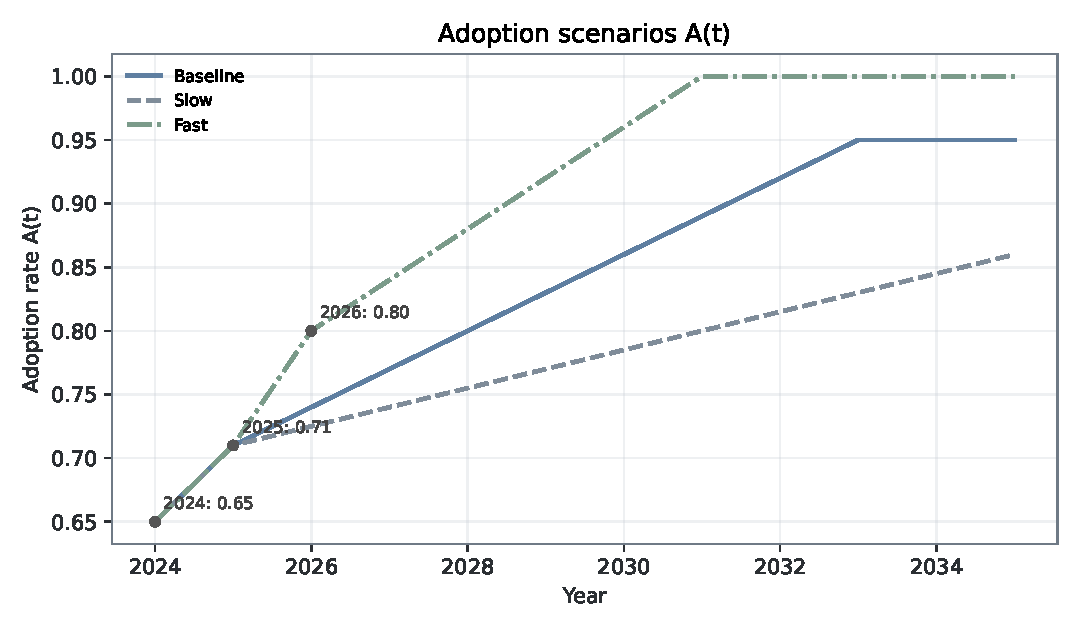
\includegraphics[width=0.85\linewidth]{figures/fig_A_t_scenarios.pdf}
\caption{基于锚点定义的GenAI采纳情景 $A(t)$（快速/中速/慢速），并标注2024--2026锚点。}
\label{fig:adoption}
\end{figure}

\paragraph{图2：顶部任务的任务劳动需求轨迹。}
\begin{figure}[H]
\centering
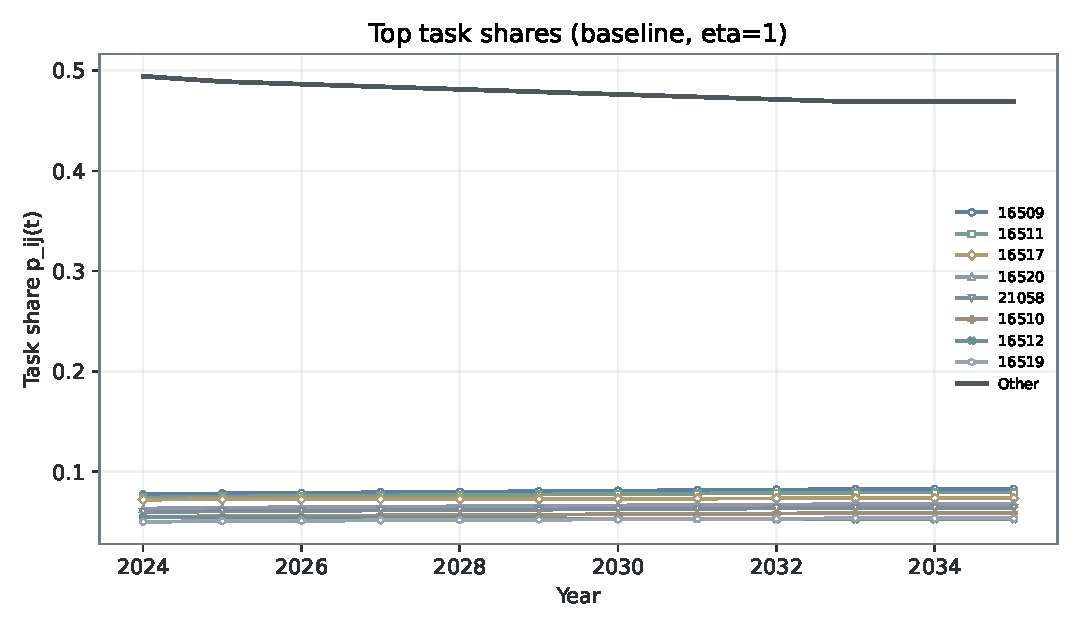
\includegraphics[width=0.95\linewidth]{figures/fig_STEM_task_share_topK.pdf}
\caption{STEM职业（17-2199.08）在基准情景下的前 $K$ 任务份额轨迹（含Other聚合），展示核心任务结构随时间的演化。}
\label{fig:task_demand_top}
\end{figure}

\paragraph{图3：任务结构漂移 $w_{ij}(t)$。}
完整任务结构演化图已在附录中给出，用于展示所有任务的份额变化（参见附录）。

\paragraph{图4：重新定义证据和触发时间 $t^*$。}
\begin{figure}[H]
\centering
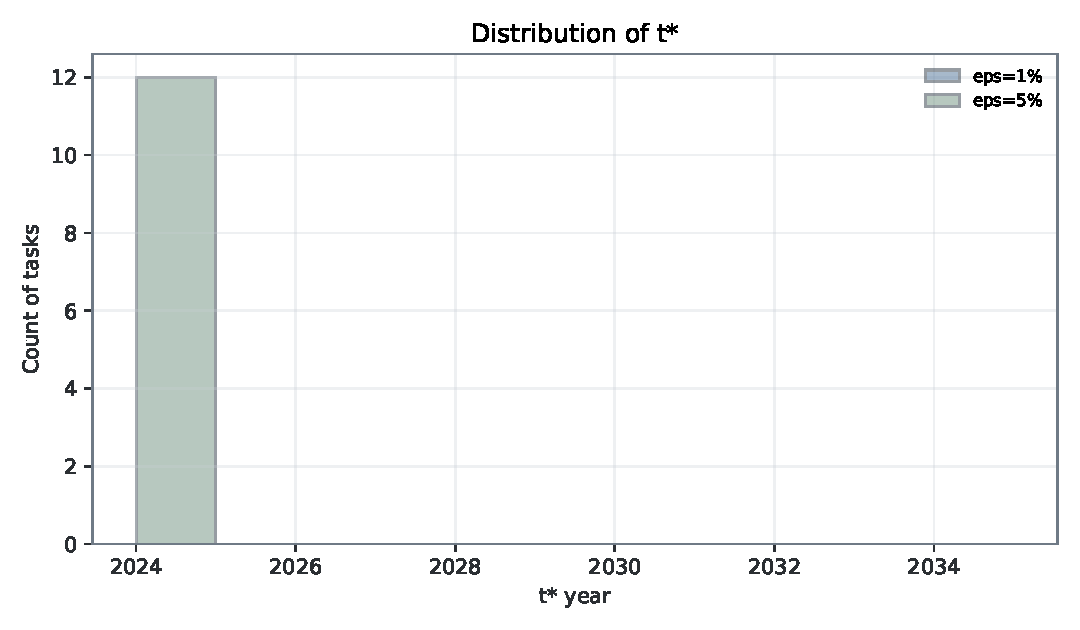
\includegraphics[width=0.95\linewidth]{figures/fig_STEM_tstar_bar.pdf}
\caption{STEM职业在基准情景下的任务“有效归零时间”分布（$\epsilon=1\%$ 与 $5\%$）。}
\label{fig:redefinition_trigger}
\end{figure}

\paragraph{图5：排名翻转的重分配证据。}
\begin{figure}[H]
\centering
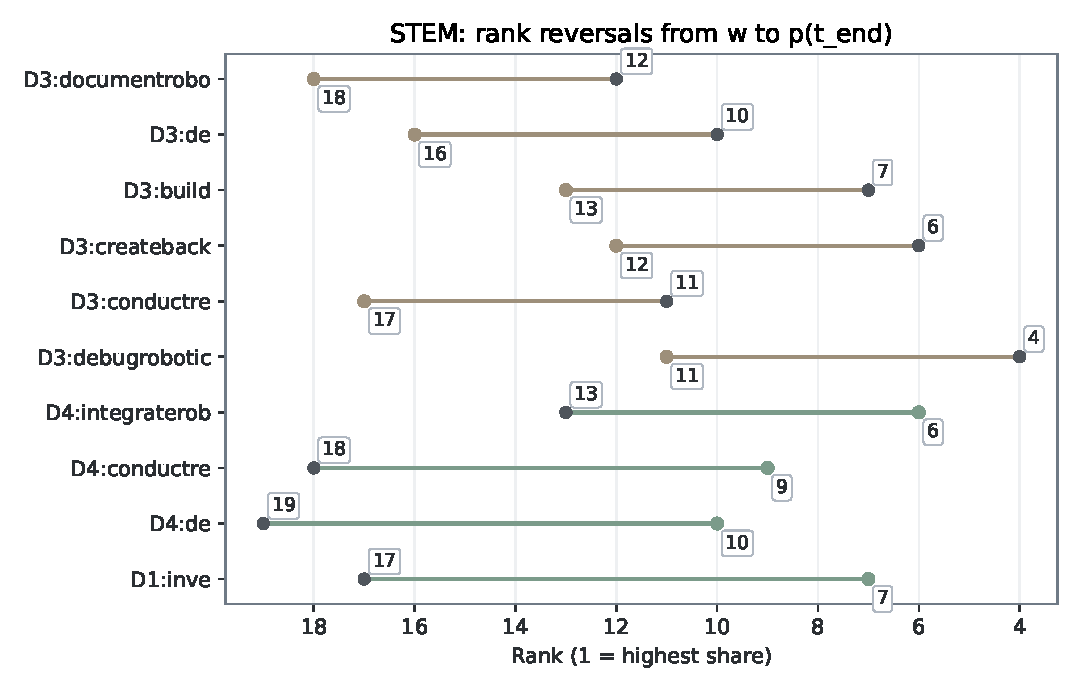
\includegraphics[width=0.95\linewidth]{figures/fig_STEM_rankflip_contribution_v2.pdf}
\caption{STEM职业（17-2199.08）从基线（$t_0=0$, $A=0$）到末期（$t_1=2040$）的排名翻转。连线两端分别为 $\mathrm{rank}_i(j,t_0)$ 与 $\mathrm{rank}_i(j,t_1)$，翻转幅度越大、线越陡，结构性重排越显著。归一化翻转强度 $\widetilde I_i$ 标注于图中。}
\label{fig:rank_flip_stem}
\end{figure}

\paragraph{图6：Top contributors 贡献分解瀑布图。}
\begin{figure}[H]
\centering
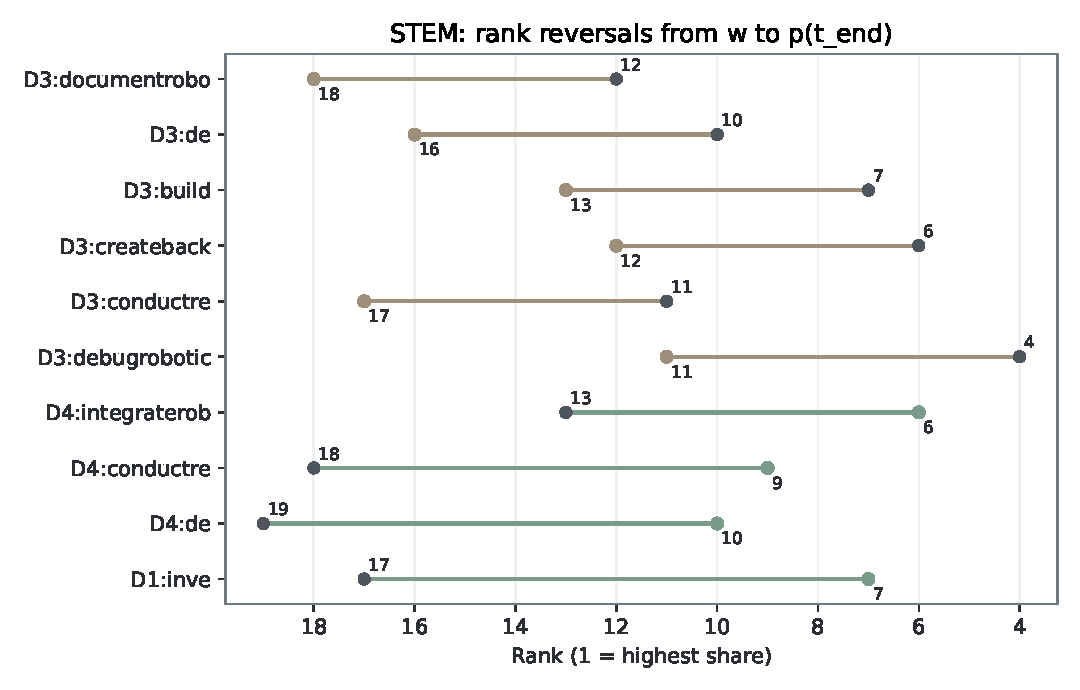
\includegraphics[width=0.95\linewidth]{figures/fig_STEM_waterfall_contribution.pdf}
\caption{STEM职业（17-2199.08）结构变化的 Top contributors 贡献分解。按 $r_{ij}$ 降序展示各任务对总份额变化的累积贡献，正值（增）与负值（减）分别标注，揭示结构重排的主要驱动任务。}
\label{fig:waterfall}
\end{figure}


\subsection{敏感性与稳健性}
\label{sec:sensitivity}

\subsubsection{低置信度任务敏感性}
\label{sec:low_conf_task}
由于与权威评估维度的语义匹配较弱，某些任务可能具有低置信度的 $(s_{ij},c_{ij})$ 分配。对于每个标记的任务，我们运行两种有界敏感性情况：
\begin{itemize}
  \item \textbf{删除：} 从集合中移除该任务，并重新归一化剩余的 $w_{ij}(0)$。
  \item \textbf{重新标记：} 保持 $w_{ij}(0)$，但用第二最佳可接受映射（或保守界限）替换 $(s_{ij},c_{ij})$。
\end{itemize}
我们报告以下变化：(i) 重新定义是否在范围内发生，(ii) 触发时间 $t^*$，以及 (iii) 消亡质量曲线 $M_{\text{drop}}(t)$。

\subsubsection{关键参数敏感性}
\label{sec:param_sens}
我们仅变化最小、高杠杆的参数集以避免过拟合：
\begin{itemize}
  \item $\kappa_s$（替代速度）：慢速/中速/快速值。
  \item $\kappa_c$（规模化开/关）：$\kappa_c=0$ 与正值。
  \item 阈值 $(\varepsilon,\theta,\delta)$：保守与激进设置。
\end{itemize}
对于每种组合，我们总结定性结论的稳定性（哪些任务变得可忽略不计，以及是否/何时触发重新定义）。

\subsection{输出摘要模板（每个职业）}
\label{sec:output_template}
对于每个职业和每个采纳情景，我们呈现：
\begin{enumerate}
  \item \textbf{任务需求结果：} 按 $D_{ij}(15)/D_{ij}(0)$ 排名的任务列表，突出显示低于 $\varepsilon$ 的任务。
  \item \textbf{任务结构变化：} $w_{ij}(t)$ 的可视化以及漂移度量 $\mathrm{JS}(w_i(t)\|w_i(0))$。
  \item \textbf{重新定义决策：} 结构指标 $\widetilde I_i$ 或 $J_i$ 是否超过阈值（\eqref{eq:redefinition_trigger}），并辅以消亡质量 \eqref{eq:Mdrop} 进行验证。
\end{enumerate}
